\documentclass[a4paper, 12pt]{article}

\usepackage[utf8]{inputenc}
\usepackage[brazil]{babel}
\usepackage[top=2cm, bottom=2cm, left=3cm, right=2cm]{geometry}
\usepackage{graphicx}
\usepackage{float}
%\usepackage{helvet}
%\renewcommand{\familydefault}{\sfdefault}



\newtheorem{defi}[subsection]{Definição}

\begin{document}
    \begin{center}
        \Large UNIVERSIDADE FEDERAL DE SERGIPE\\CENTRO DE CIÊNCIAS EXATAS E DA TERRA\\DEPARTAMENTO DE FÍSICA
        \vspace{50mm}
        
        \normalsize
        \textbf{Victor S. Nunes}
        \vspace{60mm}
        
        \Large \textbf{Modelo de TCC escrito em \LaTeX}
        \vspace{100mm}
        
        \normalsize
        São Cristóvão, 01 de Janeiro de 2020
        \thispagestyle{empty}
    \end{center}
    \newpage
    \begin{center}
        \Large Victor S. Nunes
        \vspace{50mm}
        
        MODELO DE TCC ESCRITO EM \LaTeX
    \end{center}
    \vspace{50mm}
    
    \begin{flushright}
        Trabalho de Conclusão de Curso submetido à\\Universidade Federal de Sergipe como requisito\\para receber o grau de bacharel em Astrofísica
    \end{flushright}
    \vspace{100mm}
    
    \begin{center}
        São Cristóvão, 01 de Janeiro de 2020
    \end{center}
    \thispagestyle{empty}
    
    \newpage
    
    \abstract{Lorem ipsum dolor sit amet, consectetur adipiscing elit. Proin turpis enim, ultricies sit amet ante non, consectetur elementum nisi. Praesent dictum condimentum scelerisque. Cras nibh massa, facilisis vel tristique at, facilisis a tellus. Aliquam vitae gravida nibh. Vestibulum ornare pretium mauris et congue. Maecenas vehicula consequat mauris accumsan suscipit. Maecenas vulputate, leo sed gravida vestibulum, erat nulla mattis massa, et volutpat quam libero id dui. Vivamus eleifend dui neque, quis convallis tellus condimentum nec. Quisque mi nisi, cursus vel nisi eget, laoreet finibus elit. }
    \thispagestyle{empty}
    
    \newpage
    \listoffigures
    \pagenumbering{roman}    
    \setcounter{page}{1}
    
    \newpage
    \listoftables
    
    \newpage
    \tableofcontents
    \thispagestyle{empty}
    
    \newpage
    
    \pagenumbering{arabic}    
    \setcounter{page}{1}
    
    \newpage
    \section{Introdução}
     Lorem ipsum dolor sit amet, consectetur adipiscing elit. Proin turpis enim, ultricies sit amet ante non, consectetur elementum nisi. Praesent dictum condimentum scelerisque. Cras nibh massa, facilisis vel tristique at, facilisis a tellus. Aliquam vitae gravida nibh. Vestibulum ornare pretium mauris et congue. Maecenas vehicula consequat mauris accumsan suscipit. Maecenas vulputate, leo sed gravida vestibulum, erat nulla mattis massa, et volutpat quam libero id dui. Vivamus eleifend dui neque, quis convallis tellus condimentum nec. Quisque mi nisi, cursus vel nisi eget, laoreet finibus elit.
\begin{quote}
Maecenas eu volutpat turpis, in blandit nunc. Aliquam porttitor tortor eu diam mollis, et facilisis eros porttitor. Aenean purus ligula, molestie nec neque vestibulum, sagittis faucibus lectus. Cras sit amet ante sed diam ornare ultrices vitae ac justo. Nunc nec imperdiet est, eget bibendum nisl. Sed consectetur risus viverra auctor aliquet. Etiam quis rhoncus ante.    
\end{quote}

Nulla sit amet lectus et sapien pretium eleifend. Nam pharetra, urna et porttitor auctor, ipsum sapien rutrum ligula, id porttitor sem lacus nec nulla. Donec imperdiet iaculis urna ut dapibus. Maecenas pulvinar semper ipsum sagittis fermentum. Fusce bibendum vestibulum volutpat. Vestibulum ante ipsum primis in faucibus orci luctus et ultrices posuere cubilia curae; Donec ac sem gravida, egestas lacus ac, molestie tortor. Lorem ipsum dolor sit amet, consectetur adipiscing elit. Sed gravida semper viverra. Vestibulum venenatis dolor eu augue tincidunt, a egestas sapien eleifend. Aliquam erat volutpat. \cite{boas2006mathematical}

\subsection{Problemas}
Cras quis justo quis quam dapibus rhoncus non vitae lacus. Morbi dictum lobortis quam ac dapibus. Pellentesque vitae diam tortor. Maecenas nec tincidunt lacus. Suspendisse egestas, augue a egestas rutrum, ipsum erat aliquet elit, euismod rutrum arcu justo tristique diam. Pellentesque aliquet luctus diam, ut iaculis nunc. Maecenas mollis facilisis risus in iaculis. Sed tempus viverra turpis eu rutrum. Phasellus accumsan purus nec nulla sollicitudin, ut aliquet dui egestas. Vivamus venenatis, arcu ut dignissim vestibulum, mauris mauris elementum felis, nec dictum sapien augue at ante. Nulla commodo finibus tellus, eget euismod dolor vestibulum in. 
    
    \section{Objetivos}
    \subsection{Objetivos Gerais}
Maecenas eu volutpat turpis, in blandit nunc. Aliquam porttitor tortor eu diam mollis, et facilisis eros porttitor. Aenean purus ligula, molestie nec neque vestibulum, sagittis faucibus lectus. Cras sit amet ante sed diam ornare ultrices vitae ac justo. Nunc nec imperdiet est, eget bibendum nisl. Sed consectetur risus viverra auctor aliquet. Etiam quis rhoncus ante. 
\newpage
\subsection{Objetivos Específicos}
\begin{itemize}
    \item Nulla sit amet lectus et sapien pretium eleifend. Nam pharetra, urna et porttitor auctor, ipsum sapien rutrum ligula, id porttitor sem lacus nec nulla.
    \item Nulla sit amet lectus et sapien pretium eleifend. Nam pharetra, urna et porttitor auctor, ipsum sapien rutrum ligula, id porttitor sem lacus nec nulla.
\end{itemize}
    
    \section{Metodologia}
    \begin{enumerate}
    \item Maecenas eu volutpat turpis, in blandit nunc. Aliquam porttitor tortor eu diam mollis, et facilisis eros porttitor. Aenean purus ligula, molestie nec neque vestibulum, sagittis faucibus lectus. Cras sit amet ante sed diam ornare ultrices vitae ac justo. Nunc nec imperdiet est, eget bibendum nisl. Sed consectetur risus viverra auctor aliquet. Etiam quis rhoncus ante. 
    \item Maecenas eu volutpat turpis, in blandit nunc. Aliquam porttitor tortor eu diam mollis, et facilisis eros porttitor. Aenean purus ligula, molestie nec neque vestibulum, sagittis faucibus lectus. Cras sit amet ante sed diam ornare ultrices vitae ac justo. Nunc nec imperdiet est, eget bibendum nisl. Sed consectetur risus viverra auctor aliquet. Etiam quis rhoncus ante. 
\end{enumerate}
    
    \section{Leis de Maxwell}
    Nulla sit amet lectus et sapien pretium eleifend. Nam pharetra, urna et porttitor auctor, ipsum sapien rutrum ligula, id porttitor sem lacus nec nulla. Donec imperdiet iaculis urna ut dapibus. Maecenas pulvinar semper ipsum sagittis fermentum. Fusce bibendum vestibulum volutpat. Vestibulum ante ipsum primis in faucibus orci luctus et ultrices posuere cubilia curae.

\begin{defi}
(Exemplo) Sed sagittis nisl enim, eu pretium metus pharetra quis. Nunc eleifend lectus a nisl ultricies finibus. Morbi ut ultricies neque. Curabitur sagittis vestibulum mi, nec auctor diam ultricies id. Morbi tincidunt nisl leo, sed efficitur est mattis vitae. Aliquam erat volutpat. Nam fringilla tristique orci rutrum tempus. 
\end{defi}

Maecenas eu volutpat turpis, in blandit nunc. Aliquam porttitor tortor eu diam mollis, et facilisis eros porttitor. Aenean purus ligula, molestie nec neque vestibulum, sagittis faucibus lectus. Cras sit amet ante sed diam ornare ultrices vitae ac justo. Nunc nec imperdiet est, eget bibendu

\begin{figure}[!htb]
    \centering
    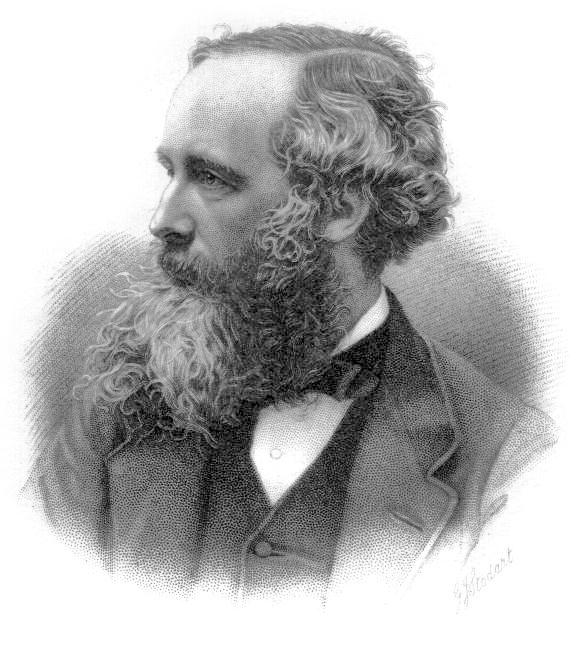
\includegraphics[width=0.3\linewidth]{James_Clerk_Maxwell_big.jpg}
    \caption{James Maxwell}
    \label{fig:maxwell}
\end{figure}

\newpage

Nulla sit amet lectus et sapien pretium eleifend. Nam pharetra, urna et porttitor auctor, ipsum sapien rutrum ligula, id porttitor sem lacus nec nulla. 

\begin{description}
    \item[Lei de Gauss]
    $$\nabla \cdot \textbf{E} = \frac{\rho}{\epsilon_{0}}$$
    
    \item[Lei de Gauss para o Magnetismo]
    $$\nabla \cdot \textbf{B} = 0$$
    
    \item[Lei de Faraday para Indução]
    $$\nabla \times \textbf{E} = -\frac{\partial \textbf{B}}{\partial t}$$
    
    \item[Lei circular de Ampère]
    $$\nabla \times \textbf{B} = \mu_{0}\left(\textbf{J} + \epsilon_{0}\frac{\partial \textbf{E}}{\partial t} \right)$$
\end{description}

\newpage
    
    \section{Aplicações do Eletromagnetismo}
    \subsection{Máquinas Eletromagnéticas}
\subsubsection{Transformadores}
Lorem ipsum dolor sit amet, consectetur adipiscing elit. Proin turpis enim, ultricies sit amet ante non, consectetur elementum nisi. Praesent dictum condimentum scelerisque. Cras nibh massa, facilisis vel tristique at, facilisis a tellus. Aliquam vitae gravida nibh. Vestibulum ornare pretium mauris et congue. Maecenas vehicula consequat mauris accumsan suscipit. Maecenas vulputate, leo sed gravida vestibulum, erat nulla mattis massa, et volutpat quam libero id dui. Vivamus eleifend dui neque, quis convallis tellus condimentum nec. Quisque mi nisi, cursus vel nisi eget, laoreet finibus elit. 

\begin{figure}[!htb]
    \centering
    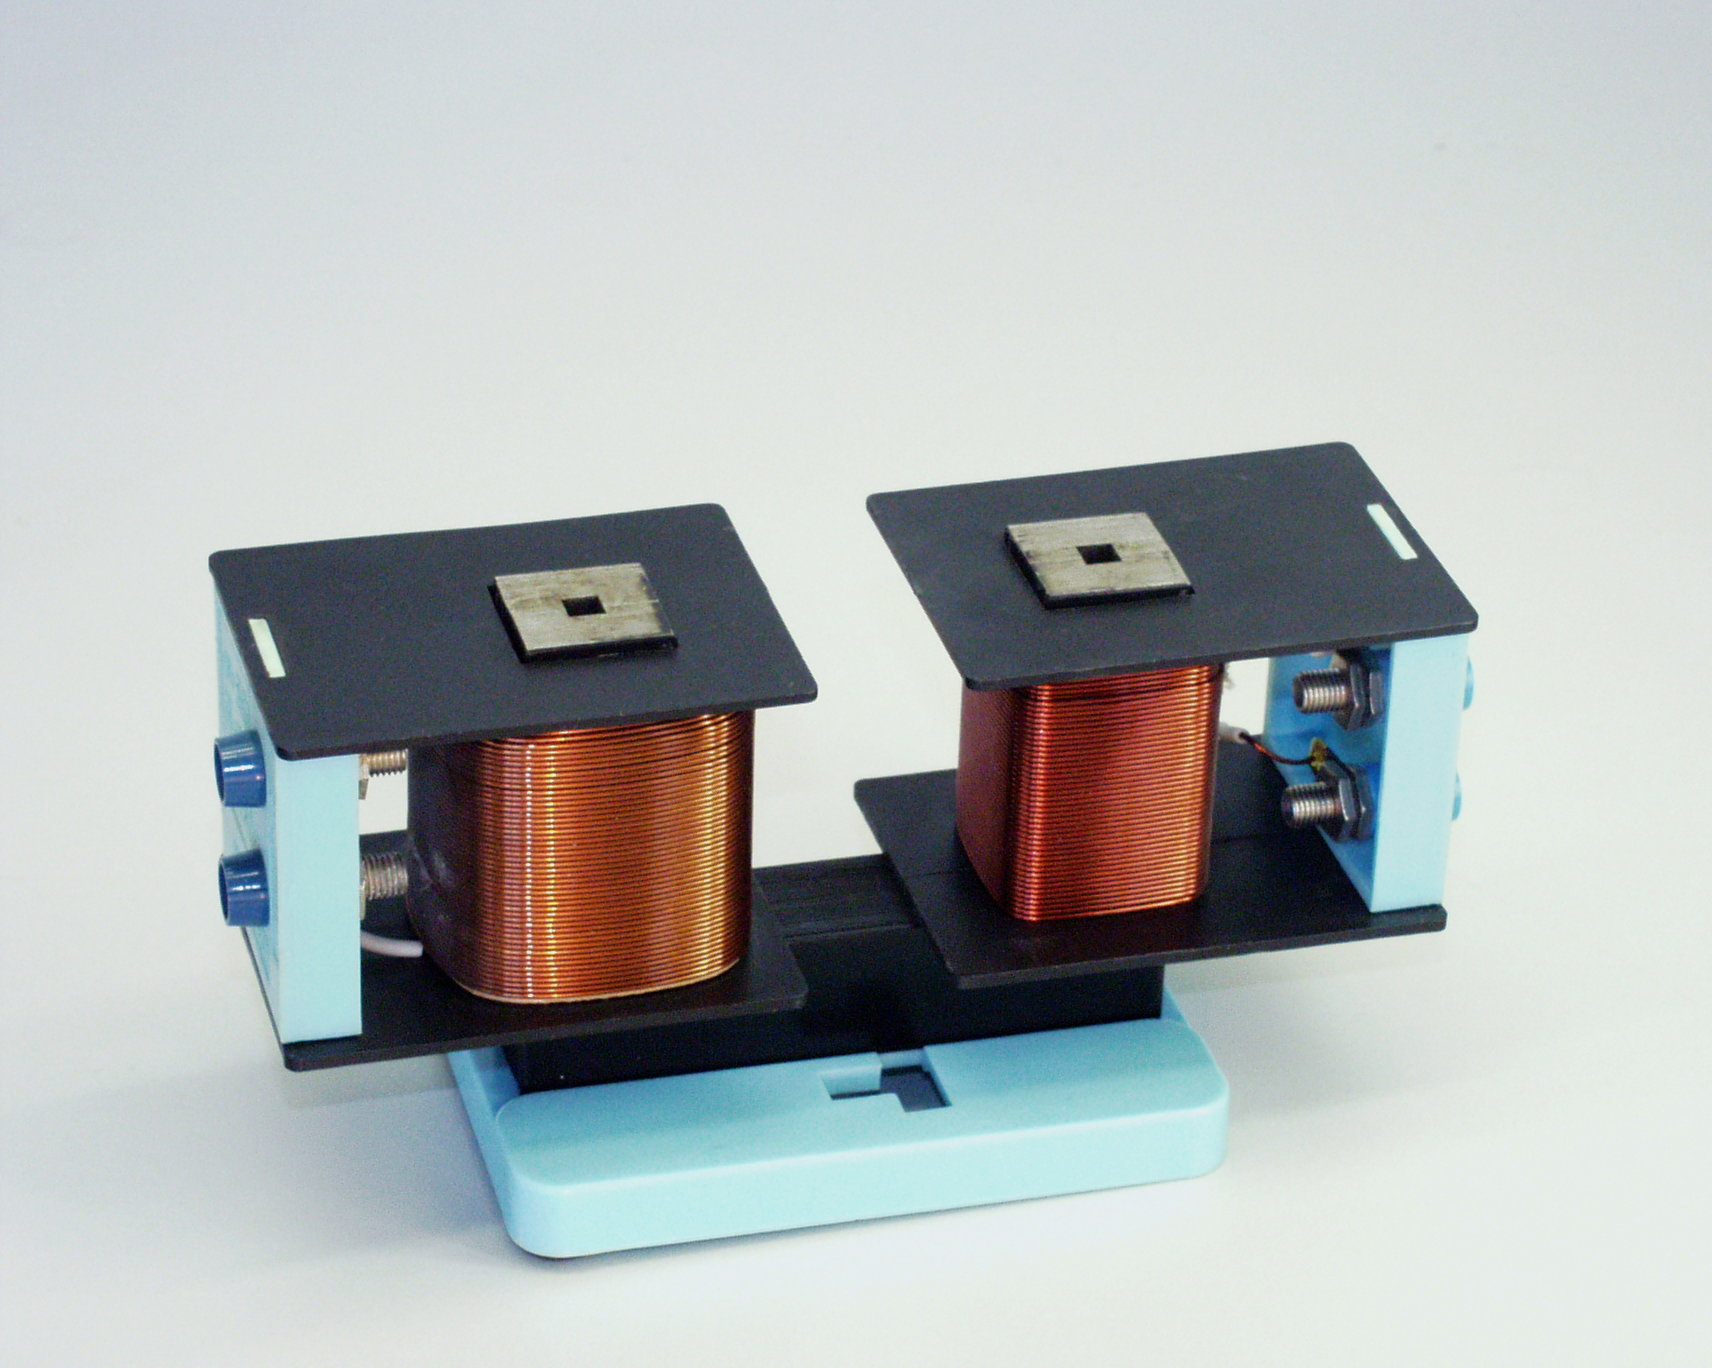
\includegraphics[scale=0.2]{Trafo_3.jpg}
    \caption{Transformador}
    \label{fig:trafo}
\end{figure}
    
    \section{Resultados}
    \subsection{Resultados Experimentais}
\subsubsection{Relação Resistência/Tensão}
Maecenas eu volutpat turpis, in blandit nunc. Aliquam porttitor tortor eu diam mollis, et facilisis eros porttitor. Aenean purus ligula, molestie nec neque vestibulum, sagittis faucibus lectus. 

\begin{figure}[!htb]
    \centering
    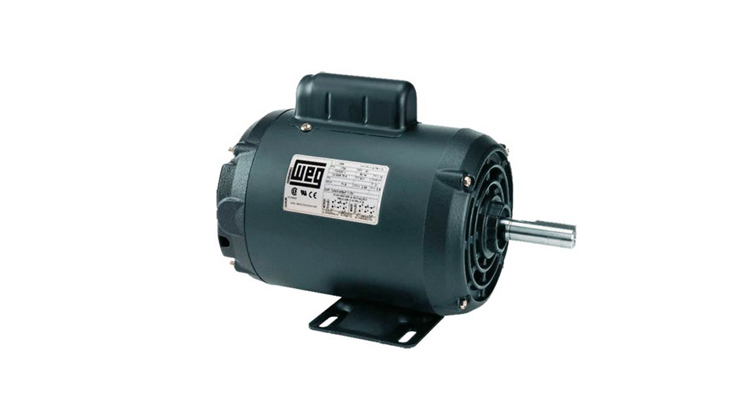
\includegraphics[scale=0.1]{motor_mono.jpg}
    \caption{Motor Monofásico}
    \label{fig:motor}
\end{figure}

Nulla sit amet lectus et sapien pretium eleifend. Nam pharetra, urna et porttitor auctor, ipsum sapien rutrum ligula, id porttitor sem lacus nec nulla. Donec imperdiet iaculis urna ut dapibus. Maecenas pulvinar semper ipsum sagittis fermentum. Fusce bibendum vestibulum volutpat. Vestibulum ante ipsum primis in faucibus orci luctus et ultrices posuere cubilia curae; Donec ac sem gravida, egestas lacus ac, molestie tortor. Lorem ipsum dolor sit amet, consectetur adipiscing elit. Sed gravida semper viverra. Vestibulum venenatis dolor eu augue tincidunt, a egestas sapien eleifend. Aliquam erat volutpat. 

\begin{table}[!htb]
    \centering
    \begin{tabular}{c|c}
    \hline
    Resistência & Tensão \\ \hline
    $20 \Omega$ & 2V \\
    $10 \Omega$ & 4V \\
    $0.5\Omega$ & 100V \\ \hline
    \end{tabular}
    \caption{Relação resistência/Tensão}
    \label{tab:relação res/ten}
\end{table}

\subsection{Relação Corrente/Luminosidade}
Maecenas eu volutpat turpis, in blandit nunc. Aliquam porttitor tortor eu diam mollis, et facilisis eros porttitor. Aenean purus ligula, molestie nec neque vestibulum, sagittis faucibus lectus. Cras sit amet ante sed diam ornare ultrices vitae ac justo. Nunc nec imperdiet est, eget bibendum nisl. Sed consectetur risus viverra auctor aliquet. Etiam quis rhoncus ante. 
\begin{table}[!htb]
\centering
\begin{tabular}{|c|c|}
\hline
Corrente & Luminosidade \\ \hline
2A       & 1lm          \\ \hline
3A       & 3lm          \\ \hline
4A       & 5lm          \\ \hline
5A       & 7lm          \\ \hline
6A       & 10lm         \\ \hline
\end{tabular}
\caption{Relação Corrente Luminosidade}
\label{tab:Relação corrente lum}
\end{table}

\subsubsection{Nota dos Materiais}
Maecenas eu volutpat turpis, in blandit nunc. Aliquam porttitor tortor eu diam mollis, et facilisis eros porttitor. Aenean purus ligula, molestie nec neque vestibulum, sagittis faucibus lectus. Cras sit amet ante sed diam ornare ultrices vitae ac justo. Nunc nec imperdiet est, eget bibendum nisl. Sed consectetur risus viverra auctor aliquet. Etiam quis rhoncus ante. 

\begin{table}[!htb]
\centering
\caption{Nota dos Materiais}
\begin{tabular}{lllll}
\hline
\multicolumn{1}{|l|}{} & \multicolumn{1}{l|}{Metal} & \multicolumn{1}{l|}{Polímero} & \multicolumn{1}{l|}{Cerâmica} & \multicolumn{1}{l|}{Semicondutor} \\ \hline
Tensão                 & 10                         & 0                             & 0                             & 7                                 \\
Corrente               & 10                         & 0                             & 0                             & 9                                 \\
Luminosidade           & 10                         & 8                             & 2                             & 0                                
\end{tabular}
\label{tab:nota dos materiais}
\end{table}

\subsection{Resultados Teóricos}
Nulla sit amet lectus et sapien pretium eleifend. Nam pharetra, urna et porttitor auctor, ipsum sapien rutrum ligula, id porttitor sem lacus nec nulla. Donec imperdiet iaculis urna ut dapibus. Maecenas pulvinar semper ipsum sagittis fermentum. Fusce bibendum vestibulum volutpat. Vestibulum ante ipsum primis in faucibus orci luctus et ultrices posuere cubilia curae; Donec ac sem gravida, egestas lacus ac, molestie tortor. Lorem ipsum dolor sit amet, consectetur adipiscing elit. Sed gravida semper viverra. Vestibulum venenatis dolor eu augue tincidunt, a egestas sapien eleifend. Aliquam erat volutpat. 

$$
    \zeta = \left( \begin{array}{cc}
        2\tau & 7\phi-\frac{5}{12} \\
        3 \psi & \frac{\pi}{8}
    \end{array} \right)
    
$$
    
    \nocite{thornton2004classical}
    \nocite{johntaylor2005}
    \nocite{eisberg1979fisica}
    \nocite{griffiths2017introduction}
    \nocite{ness1983understanding}
    
    \newpage
    \addcontentsline{toc}{section}{Referências}
    \bibliographystyle{abbrv}
    \bibliography{refs}
    
\end{document}